\documentclass[11pt, oneside]{article}   	% use "amsart" instead of "article" for AMSLaTeX format
\usepackage{geometry}                		% See geometry.pdf to learn the layout options. There are lots.
\geometry{letterpaper, margin=.5in}                   		% ... or a4paper or a5paper or ... 
%\geometry{landscape}                		% Activate for rotated page geometry
%\usepackage[parfill]{parskip}    		% Activate to begin paragraphs with an empty line rather than an indent
\usepackage{graphicx}				% Use pdf, png, jpg, or eps§ with pdflatex; use eps in DVI mode
								% TeX will automatically convert eps --> pdf in pdflatex		
\usepackage{wrapfig}								
\usepackage{amssymb}
%SetFonts
%SetFonts
\date{}							% Activate to display a given date or no date

\begin{document}

\section*{Part A}
\begin{wrapfigure}[18]{r}{0.5\textwidth}
\begin{flushright}
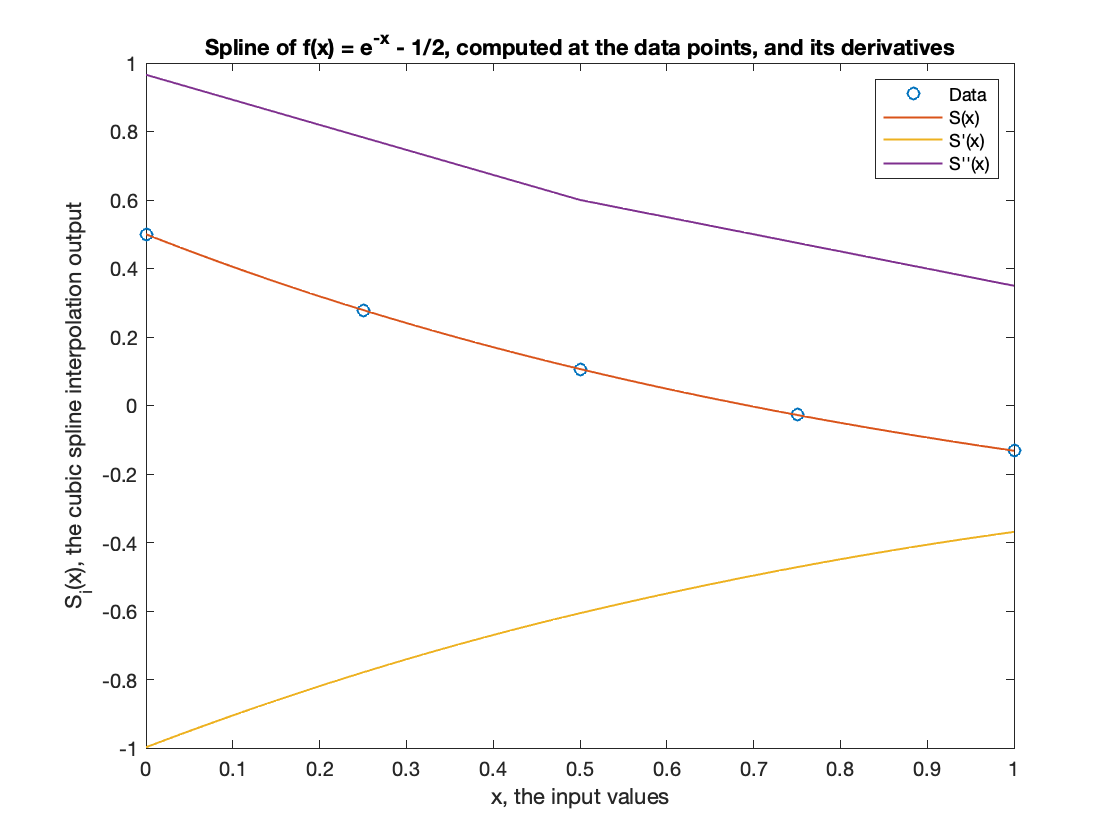
\includegraphics [scale=.25] {PartA.png}
\end{flushright}
\end{wrapfigure}

The function $f(x) = e^{-x} - \frac{1}{2}$, evaluated at $x = 0, 0.25, 0.5, 0.75, 1$, is given by the circular data points. From this data, a cubic spline with not-a-knot end conditions was constructed, and its first and second derivatives were computed. Each is shown for reference.\\

Since the spline is cubic, it has the form $S_i(x) = a_i + b_ix + c_ix^2 + d_ix^3$. The coefficients for the spline $S$ are as follows: \\
$~$\\
$   -0.1218  ~~  0.4828 ~~  -0.9979 ~~ 0.5000$\\
$   -0.1218  ~~ 0.3914 ~~  -0.7793  ~~  0.2788$\\
$   -0.0835  ~~  0.3001 ~~  -0.6065  ~~  0.1065$\\
$   -0.0835  ~~  0.2374 ~~  -0.4721 ~~  -0.0276$\\

From which the derivatives are simple to construct. The approximations for $f'(0.5)$ and $f''(0.5)$ are $S'(0.5) \approx -0.6065$, $S''(0.5) \approx 0.6001$, and their absolute errors are $|S'(0.5) - f'(0.5)| \approx 7.9565$e-$05$ and $|S''(0.5) - f''(0.5)| \approx 0.0064$.
\section*{Part B}
\begin{centering}
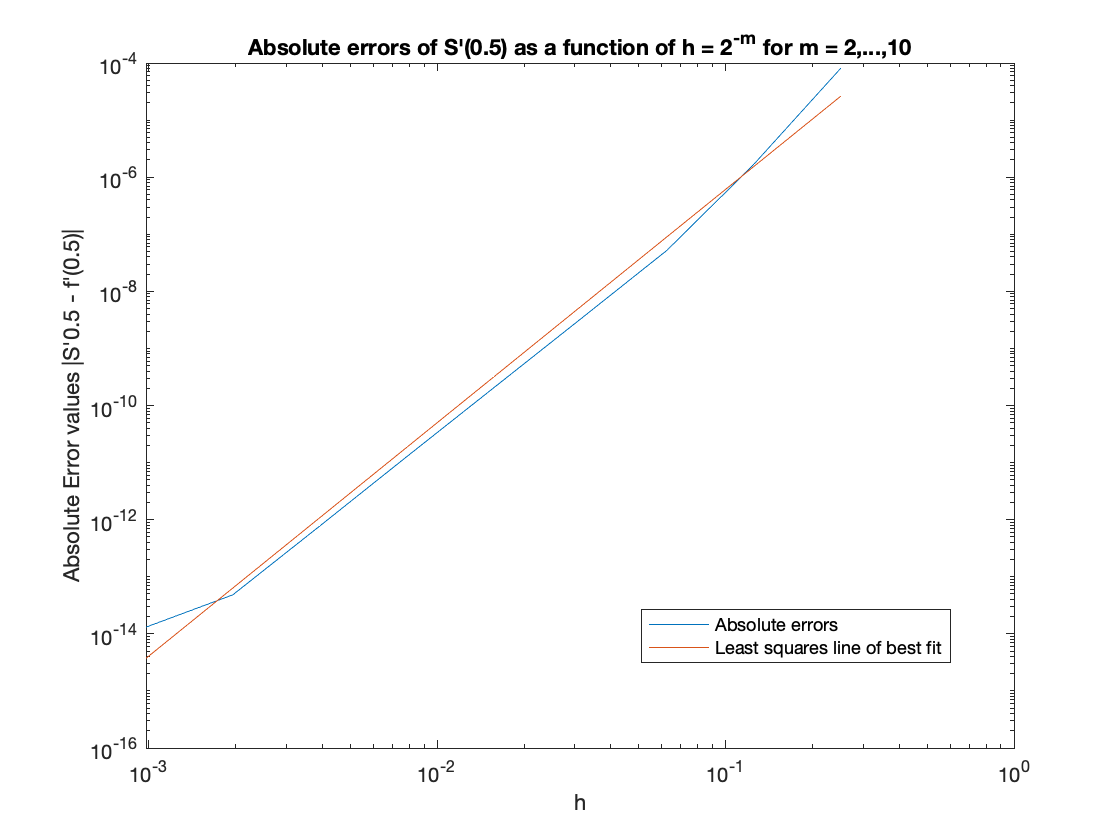
\includegraphics [scale=.25] {PartB1.png}
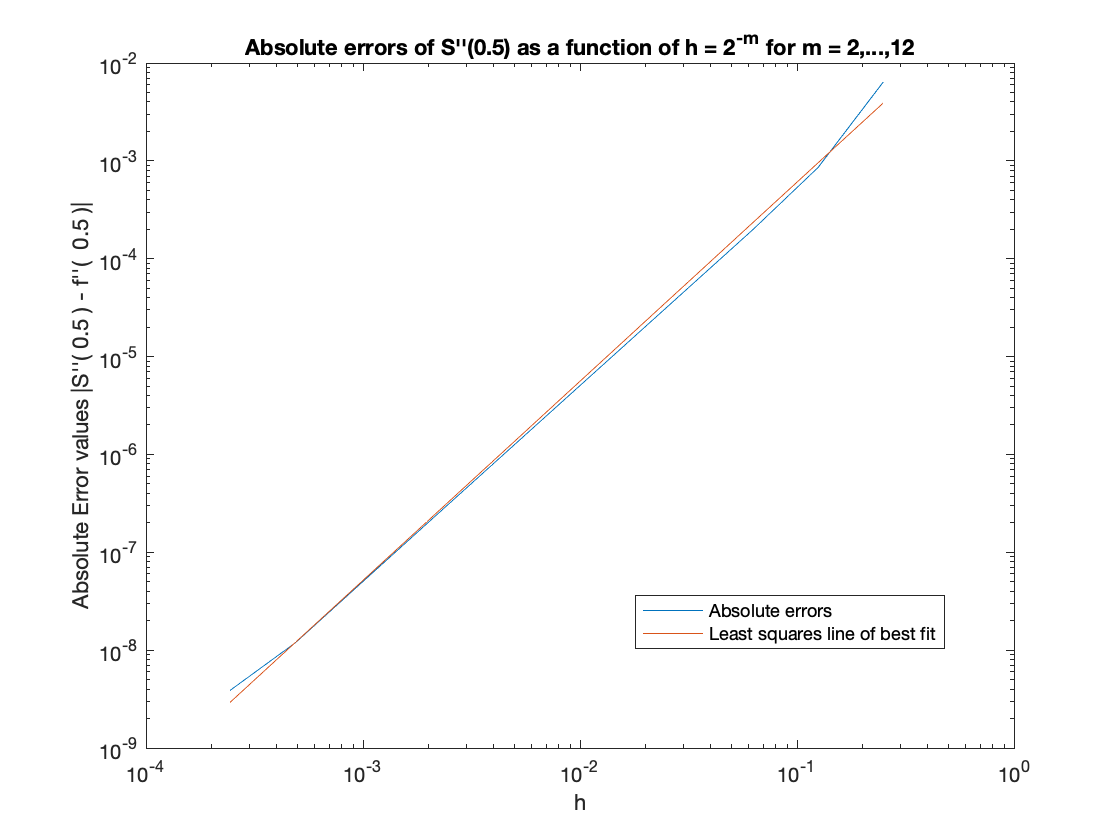
\includegraphics [scale=.25] {PartB2.png}
\end{centering}

We repeat Part A over the interval [0,1] with equal node spacings $h = 2^{-m}, m = 2, 3, ..., 10$ for the LHS plot and $m = 2, 3, ..., 12$ for the RHS plot. We limit $m$ since higher values introduce erratic behaviour. Since $error = c \cdot h^p$, solving for $p$ will allow us to describe the error in our approximations in $O$ notation. We linearize the data by plotting $\log(error) = \log (ch^p)$, for each $h = 2^{-m}$, for each of $S'(0.5)$ and $S''(0.5)$. We then approximate these lines by applying a least squares regression. Recall that these lines have the form $\log(error) = \log (c \cdot h^p) \Rightarrow \log(error) = \log(c) + p \log(h)$. Solving for the slope, $p$, allows us to describe the error, as desired:\\
$~$\\
The error in the approximations for $f'(0.5) \approx S'(0.5)$ as a function of $h$ are $O(h^{4.087})$, thus $p \approx 4.087$.\\
The error in the approximations for $f''(0.5) \approx S''(0.5)$ as a function of $h$ are $O(h^{2.035})$, thus $p \approx 2.035$.\\
\end{document}  